\documentclass{standalone}
\usepackage{tikz}
\usetikzlibrary{calc,math,decorations.pathreplacing}


\begin{document}
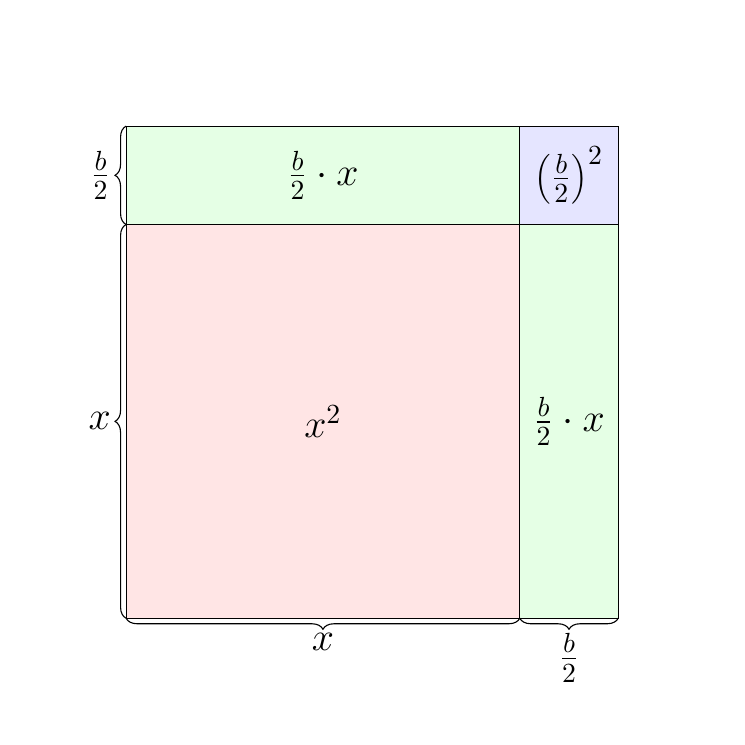
\begin{tikzpicture}[scale=2.5]

    \tikzmath{\size = 3;}
    % selecting the first quadrant
    \clip (-0.5,-0.5) rectangle (\size,\size);
    % setting up the Cartesian Grid. Note "help lines" = "gray, very thin"
    %\draw[step=.5cm,help lines] (-1.6,-1.6) grid (\size,\size); 

    % draw the process of completing the square
    \draw[fill=red!20, fill opacity=0.5] (0,0) rectangle (2,2) node[pos=.5, fill opacity=1] {\Large $x^2$};
    \draw[fill=green!20, fill opacity=0.5] (2,0) rectangle ++(.5,2) node[pos=.5, fill opacity=1] {\Large $\frac{b}{2}\cdot x$};
    \draw[fill=green!20, fill opacity=0.5] (0,2) rectangle ++(2,.5) node[pos=.5, fill opacity=1] {\Large $\frac{b}{2}\cdot x$};
    \draw[fill=blue!20, fill opacity=0.5] (2,2) rectangle ++(.5,.5) node[pos=.5, fill opacity=1] {\Large $\left(\frac{b}{2}\right)^2$};

    % add labels
    \draw[decorate,decoration={brace,amplitude=4pt}] (2,0) -- (0,0) node[midway,below, yshift=-2pt] {\Large $x$};
    \draw[decorate,decoration={brace,amplitude=4pt}] (0,0) -- (0,2) node[midway,left, xshift=-2pt] {\Large $x$};

    \draw[decorate,decoration={brace,amplitude=4pt}] (2.5,0) -- (2,0) node[midway,below, yshift=-2pt] {\Large $\frac{b}{2}$};
    \draw[decorate,decoration={brace,amplitude=4pt}] (0,2) -- (0,2.5) node[midway,left, xshift=-2pt] {\Large $\frac{b}{2}$};


\end{tikzpicture}
\end{document}